% !Mode:: "TeX:UTF-8"
%!TEX program  = xelatex

%\documentclass[bwprint]{cumcmthesis}
\documentclass[withoutpreface,bwprint]{cumcmthesis} %去掉封面与编号页

\title{虚功原理的应用-系泊系统设计与优化}

\begin{document}


\centerline{\textbf{\zihao{3} 虚功原理的应用-系泊系统设计与优化}}

\abs{}

\par 本文综合运用虚功原理与广义坐标系等分析力学相关知识,对于单系点系泊系统设计与优化给出了较优的方案。

\par 本文通过广义坐标和虚功原理建立了系泊系统达到平衡时的基本模型, 给出了各部件的倾斜角与作用力满足平衡条件时的方程组。通过逐步搜索计算出风速为$12m/s$和$24m/s$时的相关参数,并拟合出锚链形状表达式。

\keywords{系泊系统 \quad 广义坐标 \quad 虚功原理 \quad 非线性规划 }

\section{背景介绍}

\subsection{广义坐标\upcite{理论力学}}
\par 对于n个质点形成的力学体系,如果有k个几何约束
\begin{equation}
	\label{guangyi-1}
	f_\alpha (x,y,z,t) = 0 \qquad (\alpha = 1,2,\cdots,k)
\end{equation}
\par 那么独立坐标就减少$3n-k$个。这些独立坐标,也就是力学体系的坐标。在力学体系只受有几何约束的情形下,这些独立坐标的数目叫做力学体系的\textbf{自由度}。但对于微分约束来讲,自由度的数目则可能小于独立坐标的数目。
\par 既然只有$3n-k$个坐标是独立的,如果我们令$3n-k=s$,那么我们就可以通过公式(\ref{guangyi-1}),将$3n$个不独立的坐标用s个独立参数$q_1,q_2,\cdots,q_s$及$t$表出\upcite{3},即
\begin{equation}
	\label{guangyi-2}
\left. 
  	\begin{array}{lr}  
  	x_i = x_i (q_1,q_2,\cdots,q_s,t)\\
  	y_i = y_i (q_1,q_2,\cdots,q_s,t)\\
  	z_i = z_i (q_1,q_2,\cdots,q_s,t)\\   
	\end{array}  
\right\} \quad (i = 1,2,\cdots,n,s<3n)  
\end{equation}
或
\begin{equation}
	\label{guangyi-3}
	\textbf{r}_i = \textbf{r}_i (q_1,q_2,\cdots,q_s,t) \qquad (i = 1,2,\cdots,n,s<3n)
\end{equation}
\par 公式(\ref{guangyi-3})中$q_1,q_2,\cdots,q_s$叫做拉格朗日\textbf{广义坐标},它不一定是长度,可以是角度或者其他物理量\upcite{4},例如面积$A$、 体积$\tau$、电极化强度$P$、磁化强度$M$等等。在几何约束的情况下,广义坐标的数目和自由度的数目相等。此时$s$个广义坐标,就足以规定力学体系的位置\upcite{11}。
\subsection{虚功原理\upcite{理论力学}}
\subsubsection{实位移与虚位移}
\par 设质点按规律(\ref{shiweiyi})
\begin{equation}
	\label{shiweiyi}
	x = f_1(t),\quad y = f_2(t),\quad z = f_3(t)
\end{equation}
运动,那么在无限短的时间$\mathrm{d}t$内,质点的位移为$\mathrm{d} \textbf{r}(\mathrm{d}x,\mathrm{d}y,\mathrm{d}z)$,而且$\mathrm{d} \textbf{r} = \mathop{\textbf{r}}\limits^{\cdot} \mathrm{d}t$,或$\mathrm{d}x = \mathop{x}\limits^{\cdot} \mathrm{d}t$,$\mathrm{d}y = \mathop{y}\limits^{\cdot} \mathrm{d}t$,$\mathrm{d}z = \mathop{z}\limits^{\cdot} \mathrm{d}t$。在这种情形下,质点的位矢$\textbf{r}$或坐标$(x,y,z)$由于参数$t$改变$\mathrm{d}t$而发生变化。如果$\mathrm{d}t = 0$,即时间没有变化,则$\mathrm{d} \textbf{r} = 0$,或$\mathrm{d}x= \mathrm{d}y= \mathrm{d}z=0$。质点由于运动实际上所发生的位移叫做\textbf{实位移},并以$\mathrm{d} \textbf{r}$表示\upcite{12}。
\par 假设某一时刻$t$,质点$P$在约束所许可的情况下,发生了一个无限小的变更。这一变更,不是由于质点的运动而实际发生的。而只是想象中可能发生的位移,它只决定于质点在此时刻的位置和加在它上面的约束,而不是由于时间改变而引起的。这种位移叫做\textbf{虚位移},并以$\delta \textbf{r}$表之。由于时间$t$没有改变,故$\delta t =0$。一般来讲,在任一时刻$t$,在约束许可的情况下,质点的虚位移可以不止一个。
\subsubsection{理想约束}
\par 作用在质点上的力(包括约束反力)$F$在任意虚位移$\delta \textbf{r}$中所做的功,叫做\textbf{虚功},如果作用在一力学体系上诸约束反力在任意虚位移$\delta \textbf{r}$中所作的虚功之和为零\upcite{15},即
\begin{equation}
	\label{lixiangyueshu}
	\sum\limits_{i=1}^{n} \textbf{R}_i \cdot \delta \textbf{r}_i = 0
\end{equation}
那么这种约束叫做\textbf{理想约束}。光滑面、光滑曲线、光滑铰链、刚性杆、不可伸长的绳等都是理想约束\upcite{14}。引入虚位移的目的,就在于利用公式(\ref{lixiangyueshu})来消去这些约束反力。

\subsubsection{虚功原理}
\par 以下只讨论不可解约束的情况。设受有$k$个几何约束的某力学体系处于平衡状态,取体系中任一质点$\textbf{P}_i$,并设作用在此质点上主动力的合力为$\textbf{F}_i$,约束反力的合力为$\textbf{R}_i$,则因在此体系中每一质点都必须处于平衡状态中\upcite{16},故此时必有
\begin{equation}
	\label{xugong-1}
	\textbf{F}_i + \textbf{R}_i = 0 \qquad (i = 1,2,\cdots,n)
\end{equation}
\par 现让每一质点自它的平衡位置发生一虚位移$\delta \textbf{r}_i$,则由公式(\ref{xugong-1}),得
\begin{equation}
	\label{xugong-2}
	\textbf{F}_i \cdot \delta \textbf{r}_i+ \textbf{R}_i \cdot \delta \textbf{r}_i = 0 \qquad (i = 1,2,\cdots,n)
\end{equation}
把公式(\ref{xugong-2})中各等式相加,就得到
\begin{equation}
	\label{xugong-3}
	\sum\limits_{i=1}^{n} \textbf{F}_i \cdot \delta \textbf{r}_i+ \sum\limits_{i=1}^{n} \textbf{R}_i \cdot \delta \textbf{r}_i = 0 \qquad (i = 1,2,\cdots,n)
\end{equation}
但如为理想约束\upcite{4},则根据公式(\ref{lixiangyueshu}),$\sum\limits_{i=1}^{n} \textbf{R}_i \cdot \delta \textbf{r}_i = 0$,因此,如果这样的力学体系处于平衡状态\upcite{18},则其\textbf{平衡条件}是
\begin{equation}
	\label{xugong-4}
	\delta W = \sum\limits_{i=1}^{n} \textbf{F}_i \cdot \delta \textbf{r}_i = 0
\end{equation}
或
\begin{equation}
	\label{xugong-5}
	\delta W = \sum\limits_{i=1}^{n} (\textbf{F}_{ix} \delta x_i + \textbf{F}_{iy} \delta y_i + \textbf{F}_{iz} \delta z_i) = 0
\end{equation}
\par 反之,也可以证明,如果平衡位置是约束所允许的位置,则当公式(\ref{xugong-4})对任意$\delta \textbf{r}_i$都成立时,系统在该位置必保持平衡\upcite{5}。由此可知,受有理想约束的力学体系平衡的充要条件是此力学体系的诸主动力在任意虚位移中所做的元功之和等于零。该关系叫做\textbf{虚功原理},也叫\textbf{虚位移原理}。

\section{实际问题}

\par 近浅海观测网的传输节点由浮标系统\upcite{20}、系泊系统和水声通讯系统组成\upcite{19}(如图1所示)。某型传输节点的浮标系统可简化为底面直径2m、高2m的圆柱体,浮标的质量为1000kg。系泊系统由钢管、钢桶、重物球、电焊锚链和特制的抗拖移锚组成。锚的质量为600kg,锚链选用无档普通链环,近浅海观测网的常用型号及其参数在附表中列出。钢管共4节,每节长度1m,直径为50mm,每节钢管的质量为10kg。要求锚链末端与锚的链接处的切线方向与海床的夹角不超过16度,否则锚会被拖行,致使节点移位丢失。水声通讯系统安装在一个长1m、外径30cm的密封圆柱形钢桶内,设备和钢桶总质量为100kg。钢桶上接第4节钢管,下接电焊锚链。
\begin{figure}[h]
\small
\centering
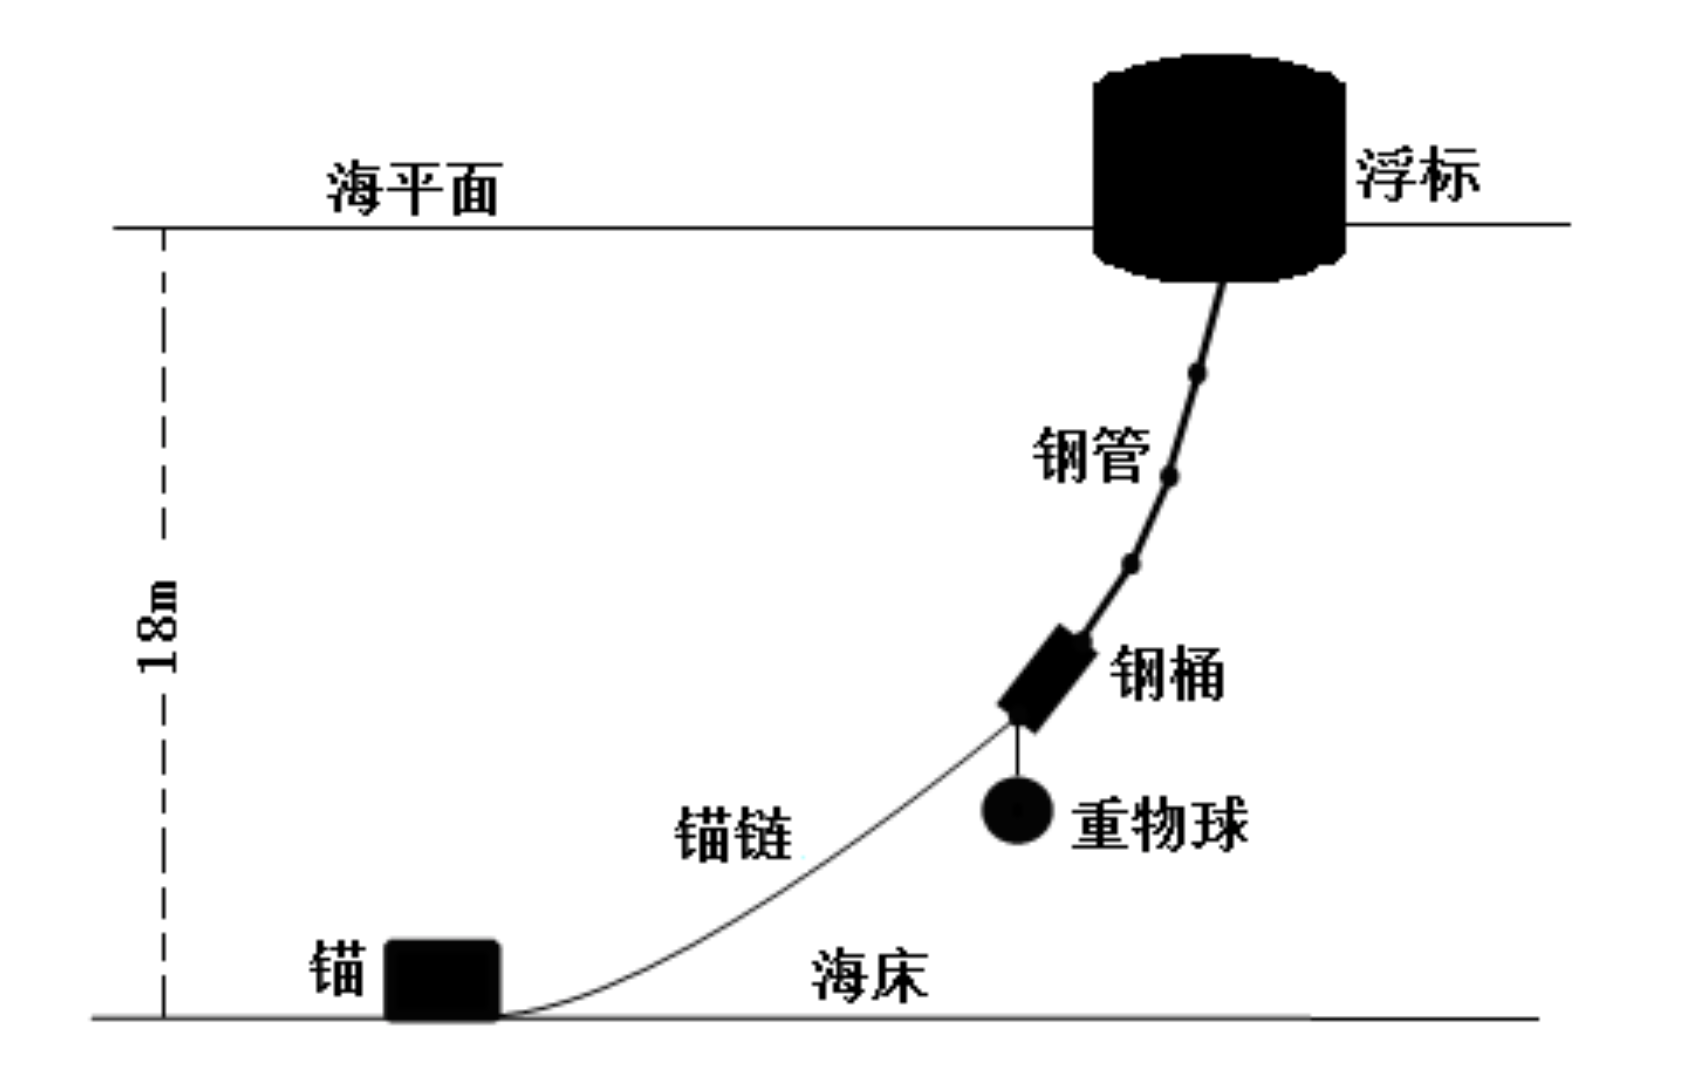
\includegraphics[width=12cm]{wentichongshu.png}
\caption{传输节点示意图} \label{fig:wentichongshu}
\end{figure}



\subsection{已知风速和和钢球质量条件下的系泊系统计算}
\subsubsection{受力分析与基本准备}
\par 通过虚功原理建立基于分析力学\upcite{6}的计算模型,将锚链的每一个链环、重物球、钢桶、四节钢管、浮标视为单独个体进行分析,最终分别求得风速为12$m/s$和24$m/s$时系泊系统的各个状态描述参数。

\par 本文分别用$f$表示浮标,$P_j$表示钢管第$j$节钢管,$D$表示钢桶, $A_k$表示锚链第$k$节锚链,$B$表示重物球。在这里,本文所考虑的主动力包括:近海面风力Ff,每个部件的重力(用$G$和部件的标号作下标表示), 海水对整个系统中各个组件的浮力(用$F$和部件的标号作下标表示)。每个部件所受主动力及建立坐标系如图(\ref{fig:zuobiaoxi})所示。

\begin{figure}[!htpb]
\small
\centering
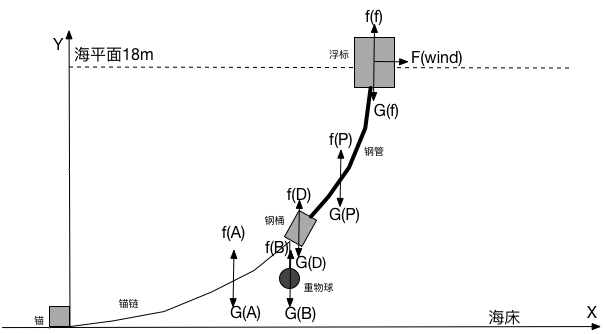
\includegraphics[width=\textwidth]{zuobiaoxi.png}
\caption{坐标系建立} \label{fig:zuobiaoxi}
\end{figure}
\subsubsection*{根据几何关系建立各组件重心与倾角关系}
\par 在广义坐标系\upcite{7}中,我们给出各个部件的重心位置和该部件与海平面间夹角的几何关系表达式如下公式(\ref{weiyifangcheng-1})所示。其中,用$y$加部件标号作为对应部件的$y$轴坐标位置,$x$加部件标号作为对应部件的$x$轴坐标位置。用$\theta$加部件标号表示该部件与海平面间夹角。
\begin{equation}
	\label{weiyifangcheng-1}
	\left\{
	\begin{array}{lr}
		y_{A1} = \frac{l_A}{2} sin \theta_{A1}\\
		y_{A2} = \frac{l_A}{2} sin \theta_{A2} + l_A sin \theta_{A1}\\
		\cdots \\
		y_{An} = \frac{l_A}{2} sin \theta_{An} + \sum\limits_{i=1}^{n-1} l_A sin \theta_{Ai}\\
		y_B = \sum\limits_{i=1}^{n} l_A sin \theta_{Ai}\\
		y_D = \frac{l_D}{2} sin \theta_D + \sum\limits_{i=1}^{n} l_A sin \theta_{Ai}\\
		y_{P1} = \frac{l_P}{2} sin \theta_{P1} + l_D sin \theta_D + \sum\limits_{i=1}^{n} l_A sin \theta_{Ai}\\
		\cdots \\
		y_{P4} = \frac{l_P}{2} sin \theta_{P4} + \sum\limits_{i=1}^{3} l_P sin \theta_{Pi} + l_D sin \theta_D + \sum\limits_{i=1}^{n} l_A sin \theta_{Ai}\\
		x_f = \sum\limits_{i=1}^{4} l_P cos \theta_{Pi} + l_D cos \theta_D + \sum\limits_{i=1}^{n} l_A cos \theta_{Ai} + \frac{1}{2} d_f + (N - n) \cdot l_A\\
		y_f = \sum\limits_{i=1}^{4} l_P sin \theta_{Pi} + l_D sin \theta_D + \sum\limits_{i=1}^{n} l_A sin \theta_{Ai} + \frac{1}{2} L_f\\
	\end{array}
	\right.
\end{equation}

\par 公式组(\ref{weiyifangcheng-1})中,$y_{Ai}$为第$i$节锚链环重心所在的纵坐标,其中$l_A$为题中所给出的第二型锚链的单节链环的长度,$\theta_{Ai}$为第$i$节锚链环与$x$轴正方向(平行于海平面)的夹角;$y_B$为金属球的球心纵坐标,可以用最后一节锚链链环的纵坐标代替;$y_D$为金属圆桶中心的纵坐标,为金属圆桶轴线与$x$轴正方向的夹角;$y_f$为浮标重心所在的纵坐标,$L_f$为浮标的高度,$d_f$为浮标的直径,$x_f$为浮标重心所在的横坐标。
\par 通过分析,我们添加如公式(\ref{y-yueshu-1})所示的约束条件,保证所有链环、钢管、钢桶在竖直方向上的投影和浮标的吃水深度($h$)之和为18$m$。
\begin{equation}
	\label{y-yueshu-1}
	\sum\limits_{i=1}^{4} l_P sin \theta_{Pi} + l_D sin \theta_D + \sum\limits_{i=1}^{n} l_A sin \theta_{Ai} + h = 18
\end{equation}

\subsubsection*{各部件所受主动力的分析}
\par 对于单个锚链链环,受到自身重力与海水对其的浮力两个主动力,其合力可由公式()求得。其中 为锚链单位长度的质量。
\begin{equation}
	\label{q1-pa}
	P_A = f_A - G_A  = \rho_w \cdot g \cdot \frac{\lambda_A \cdot l_A}{\rho_A} - \lambda_A \cdot l_A \cdot g
\end{equation}
\begin{equation}
	\label{q1-pd}
	P_D = f_D -G_D = \rho_w \cdot g \cdot (\frac{d_D}{2})^2 \pi \cdot L_D - m_D \cdot g
\end{equation}
\begin{equation}
	\label{q1-pp}
	P_P = f_P -G_P = \rho_w \cdot g \cdot (\frac{d_P}{2})^2 \pi \cdot L_P - m_P \cdot g
\end{equation}
\begin{equation}
	\label{q1-wind}
	F_{wind} = 0.625 \times S v^2
\end{equation}
\par 与单个锚链链环相似,对于钢桶竖直方向有合力$P_D$如公式(\ref{q1-pd})所示;对于钢管竖直方向有合力$P_P$如公式(\ref{q1-pp})所示;对于金属球,由于浮力对于密致金属球影响极小,因此忽略其所受到的浮力,金属球所受合力$P_B$直接由其重力表示为$P_B = G_B = m_B \cdot g$;风载荷(风力)$F_{wind}$的定义如公式(\ref{q1-wind})所示,其中$S$为迎风面积、$v$为风速。
\subsubsection*{基于虚功原理的计算}

\par 对于整个系泊系统\upcite{9},当系统达到稳定时,可以认为该系统处于一个受理想约束的力学体系中,在该体系中,所有的主动力的任意虚位移所作的所有元功之和等于零,由此得到系泊系统的平衡方程(\ref{q1-xugonyuanli})。

\begin{equation}
	\label{q1-xugonyuanli}
	\sum\limits_{i=1}^{n} P_A \cdot \delta y_{Ai} + P_D\cdot \delta y_D + \sum\limits_{i=1}^{4}P_P\cdot \delta y_{Pi} + P_B \cdot \delta y_{B} + P_f \cdot \delta y_{f} + F_{wind} \cdot \delta x_f = 0
\end{equation}

\par 在公式(\ref{q1-xugonyuanli})中,$P_A$、$P_D$、$P_P$、$P_B$、$P_f$分别表示锚链、钢桶、钢管、钢球和浮标竖直方向所受到的力,$F_{wind}$表示水平风载荷。$\delta y_{Ai}$、$\delta y_{Di}$、$\delta y_{Pi}$、$\delta y_{B}$、$\delta y_{f}$、$\delta y_{Xf}$、表示系统内各个部件分别的虚位移。
\par 将公式(\ref{q1-xugonyuanli})展开并将公式组(\ref{weiyifangcheng-1})中各个变量的计算公式代入得虚功原理计算方程\upcite{10}如公式(\ref{q1-xugong-zhankai})所示。
\begin{equation}
	\label{q1-xugong-zhankai}
	\begin{split}
		0 &= \left[ P_A \cdot \delta(\frac{l_A}{2}sin \theta_{A1}) + P_A \cdot \delta(\frac{l_A}{2}sin \theta_{A2} + l_A sin \theta_{A1}) + \cdots +P_A \cdot \delta(\frac{l_A}{2}sin \theta_{An} + \sum\limits_{i=1}^{n-1} l_A sin \theta_{Ai}) \right] \\ 
		& + P_D \cdot (\frac{l_D}{2}sin \theta_{D} + \sum\limits_{i=1}^{n}l_A sin \theta_{Ai}) + \left[ {P_P \cdot \delta(\frac{l_P}{2}sin \theta_{P1} + l_D sin \theta_D + \sum\limits_{i=1}^{n}l_A sin\theta_{Ai} ) + \cdots} \right. \\
		& \left. {+ P_P \cdot \delta(\frac{l_P}{2}sin \theta_{P4} + \sum\limits_{i=1}^{3} l_P sin \theta_{Pi} +l_D sin \theta_D \sum\limits_{i=1}^{n}l_A sin\theta_{Ai} )} \right] + P_B \cdot \delta (\sum\limits_{i=1}^{n} l_A sin \theta_{Ai}) + \\
		& P_f \cdot \delta (\sum\limits_{i=1}^{4}l_P cos\theta_{Pi} + l_D sin \theta_{D} \sum\limits_{i=1}^{n}l_A sin \theta_{Ai} + \frac{1}{2}L_f) + F_{wind} \cdot \left({\sum\limits_{i=1}^{4}l_P cos \theta_{Pi} + l_D cos \theta_D +} \right. \\
		& \left. {\sum\limits_{i=1}^{n}l_A cos \theta_{Ai} + (n-1)l_A + \frac{1}{2} d_f} \right)
	\end{split}
\end{equation}
\par 将上述公式(\ref{q1-xugong-zhankai})进行化简可得到如下公式(\ref{q1-xugong-huajian})
\begin{equation}
	\label{q1-xugong-huajian}
	\begin{split}
		0 &= l_A \sum\limits_{i=1}^{n} \left\{ { \left[(n+\frac{1}{2} - i)P_A +P_D +4P_P +P_B+P_f\right]cos \theta_{Ai} - F_{wind}sin\theta_{Ai} }\right\} \cdot \delta\theta_{Ai} + \\
		& l_D \left[ {(\frac{1}{2} P_D +4P_P+P_f)cos\theta_D - F_{wind}sin\theta_D }\right] \cdot \delta \theta_D  + \sum\limits_{i=1}^{4}l_P \left[ {(P_P(4.5-i)+P_f)cos\theta_{Pi}}\right.\\
		& \left. {-F_{wind} sin\theta_{Pi} }\right] \cdot \delta \theta_{Pi}
	\end{split}
\end{equation}
\par 由公式(\ref{q1-xugong-huajian})可以推出部件总数个方程用于求解,通过虚功原理可以得出$\delta \theta_{Ai}$、$\delta \theta_{D}$、$\delta \theta_{Pi}$是相互独立的,因此可令$\delta \theta_{Ai}$、$\delta \theta_{D}$、$\delta \theta_{Pi}$之前的系数为零,得到如下公式组(\ref{q1-xugong-qiujie}),为了简化表述,将相似方程通过循环变量$i$的形式表示。
\begin{equation}
	\label{q1-xugong-qiujie}
	\left\{
	\begin{split}
		& \left[ (n + \frac{1}{2} - i)P_A +P_D+4P_P+P_B+P_f \right] cos\theta_{Ai} - F_{wind} sin\theta_{Ai} = 0\\
		& (\frac{1}{2} P_D+4P_P+P_f)cos\theta_D - F_{wind}sin\theta_{D} = 0\\
		& \left[ P_P(4.5-i)+P_f \right] cos\theta_{Pi} - F_{wind} sin \theta_{Pi}\\
	\end{split}
	\right.
\end{equation}
由公式组(\ref{q1-xugong-qiujie})各个方程可解得系泊系统中任意部件与海平面的夹角$\theta$的表达式(\ref{q1-xugong-qiujie-2})。其中$\theta_{Ai}$为不落于海床上的第$i$节锚链环与海平面间的夹角,$\theta_D$为钢桶轴线与水平方向的夹角,$\theta_{Pi}$为第$i$节钢管于海平面的夹角。
\begin{equation}
	\label{q1-xugong-qiujie-2}
	\left\{
	\begin{split}
		& \theta_{Ai} = arctan\frac{(n + \frac{1}{2} - i)P_{Ai} +P_D+4P_P+P_B+P_f}{F_{wind}} \\
		& \theta_D = arctan\frac{\frac{1}{2}P_D+4P_P+P_f}{F_{wind}}\\
		& \theta_{Pi} = arctan\frac{P_P(4.5-i)+P_f}{F_{wind}}\\
	\end{split}
	\right.
\end{equation}
将公式组(\ref{q1-xugong-qiujie-2})中各个$\theta$的计算公式代入约束方程(\ref{rey-yueshu-1})中进行求解,得到最终结果。
\begin{equation}
	\label{rey-yueshu-1}
	\sum\limits_{i=1}^{4} l_P sin \theta_{Pi} + l_D sin \theta_D + \sum\limits_{i=1}^{n} l_A sin \theta_{Ai} + h = 18
\end{equation}


\subsubsection{该问题的求解与结果分析}
\par 锚链选择长度为$22.05m$的II型电焊锚链(锚链链环个数为210个),选用$1200kg$的重物球。求解的海域内海水密度为$1.025×10^3kg/m^3$。

\par 当海上的风速为$12m/s$时,假设$210$个锚链链环均不沉于海床面上,通过模型解得锚链,钢桶,钢管在竖直方向上的投影高度大于$18$米,不符合实际。因此$210$个锚链链环中一定有一部分锚链沉于海床面上。由于第一节锚链一定在海底,因此第一节锚链与水平方向的夹角为$0^o$。

\begin{equation}
	\label{q1-ans-1}
	\theta_{A1} = arctan\frac{(n + \frac{1}{2} - i)P_{A1} +P_D+4P_P+P_B+P_f}{F_{wind}} = 0 
\end{equation}
\par 由公式(\ref{q1-ans-1})可以求解出,此时的浮标吃水深度$h$为$0.73072$米。
\par 通过改变浮于海水中锚链链环的个数,使得锚链、钢桶、钢管在竖直方向上的投影高度等于18米。最终确定浮于海水中的锚链环的个数为$147$个(有$6.615m$的锚链沉于海床面上)。
\par 计算得到锚链、钢桶、钢管的重心坐标,得到系泊系统中各个部件的位置如下图(\ref{fig:q1-12-1})所示。
\begin{figure}[h]
\small
\centering
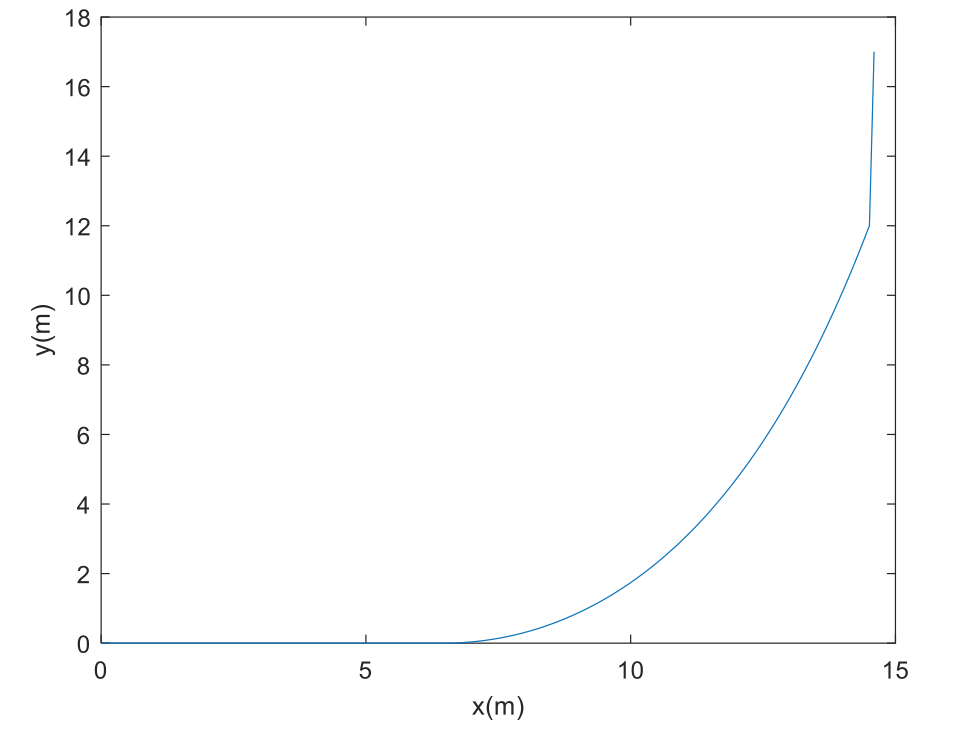
\includegraphics[width=12cm]{q1-12-1.png}
\caption{风速为$12m/s$时系泊系统各组件位置} \label{fig:q1-12-1}
\end{figure}





\section{总结}
\par 综合运用虚功原理解决实际问题,展现了物理学在社会生活中极高的应用价值。

\par 牛顿力学对每一个倾角需要使用迭代的方法,而本文采用分析力学虚功原理解释理想约束的平衡问题时,由于约束反力自动消去,可以简单的用它去求主动力在平衡时所满足的条件,即平衡条件,倾角之间是彼此相互独立的,省去了迭代步骤。



%参考文献
\begin{thebibliography}{9}%宽度9
 \bibitem{理论力学} 蔡泰信, 和兴锁, 朱西平. 理论力学[M]. 机械工业出版社, 2007.
 \bibitem{浮标} https://baike.baidu.com/item/海洋浮标/9246083?fr=aladdin
 \bibitem{3} 王焕定. 再论变形体虚功原理[J]. 力学与实践, 2011, 33(2):93-95.
 \bibitem{4} 王光远, 王焕定. 论变形体虚功原理的充分性[J]. 哈尔滨建筑大学学报, 1984(3):36-45.
 \bibitem{5} 朱昌铭. 基于虚功原理的弹性接触问题的线性互补方法[J]. 力学学报, 1995, 27(2):189-197.
 \bibitem{6} 毛坚强, 丁桂彪. 变形体的虚功原理及其在求解接触问题中的应用[J]. 西南交通大学学报, 2002, 37(3):241-245.
 \bibitem{7} 薛纭. 虚功原理与义坐标[J]. 大学物理, 2002, 21(4):3-3.
 \bibitem{8} 薛纭. 虚功原理与广义坐标[J]. 大学物理, 2002, 21(4):3-5.
 \bibitem{9} 吴惟敏. 虚功原理中的广义坐标选择[J]. 大学物理, 1991, 10(6):46-46.
 \bibitem{10} 董启莲. 虚功原理及其在工程实践中的应用[J]. 河南大学学报(自然版), 1997(2):33-36.
 \bibitem{11} 韩亚萍, 徐晓峰. 应用虚功原理时应注意的一个问题[J]. 大学物理, 2000, 19(5):22-23.
 \bibitem{12} 韩亚萍, 徐晓峰. 应用虚功原理时应注意的一个问题[J]. 大学物理, 2000, 19(5):22-23.
 \bibitem{13} 吴少平. 虚功原理及其应用[J]. 高等继续教育学报, 2000(5):24-26.
 \bibitem{14} 朱昌铭, 金永杰. 一种基于虚功原理的求解弹塑性问题的有限元——数学规划法[J]. 应用数学和力学, 1993, 14(7):601-608.
 \bibitem{15} 杜尚之. 虚功原理的应用[J]. 丽水学院学报, 1990(s1):44-48.
 \bibitem{16} 魏先祥. 虚功原理不同于最小势能原理[J]. 力学与实践, 1985, 7(4):56-58.
 \bibitem{17} 周靖. 虚功原理中的广义坐标与坐标系的选择[J]. 淮阴师范学院学报(自然科学版), 2006, 5(2):131-134.
 \bibitem{18} 涂奉生. 线性系统的广义坐标变换(II)[J]. 黑龙江大学自然科学学报, 1990(1):37-40.
 \bibitem{19} 潘斌, 高捷, 陈小红,等. 浮标系泊系统静力计算[J]. 重庆交通大学学报(自然科学版), 1997, 16(1):68-73.
 \bibitem{20} 刘海笑, 黄泽伟. 新型深海系泊系统及数值分析技术[J]. 海洋技术学报, 2007, 26(2):6-10.
  
\end{thebibliography}

\section{附录:程序}

\textbf{虚功原理计算}
% 代码插入,请将代码文件放入code文件夹,支持语言的语法高亮。支持语言:C,C++,Java,Matlab,Mathematica,python,R,可在cls文件中自行添加。
\lstinputlisting[language=Matlab]{./code/a1.m}


\end{document}